\chapter{Preliminary Vocabulary}
\label{vocab}

Before we start, there are a few uncommon terms we will use fairly often in this paper. We have briefly defined them here.

\section{Mondegreens}
\label{vocab:mondegreens}

A mondegreen is a word or phrase resulting from a misinterpretation of a word or phrase that has been heard\cite{dictionaryDotComMondegreen}.  The word was coined by American author Sylvia Wright in her article, ``The Death of Lady Mondegreen", published in a 1954 issue of Harper's Bazaar. In it, she describes the origin of the word:
\begin{quote}
When I was a child, my mother used to read aloud to me from Percy's Reliques, and one of my favorite poems began, as I remember:
    \begin{verse}
    Ye Highlands and ye Lowlands, \\
    Oh, where hae ye been? \\
    They hae slain the Earl O' Moray,\\
    And Lady \emph{Mondegreen.}
    \end{verse}

\end{quote} 
The fourth line of the quote is actually ``and laid him on the green"\cite{mondegreenOriginRef}.  

Additional commonly-cited mondegreens include:
\begin{center}
\begin{tabular}{cc}
 Gladly the Cross-Eyed Bear $\leftrightarrow$  Gladly the Cross I'd Bear\cite{gladlyTheCrossRef}  \\
 Scuse me while I kiss this guy $\leftrightarrow$  Scuse me while I kiss the sky \cite{purpleHazeRef} \\
 There's a bathroom on the right $\leftrightarrow$  There's a bad moon on the rise \cite{badMoonRisingRef} \\
\end{tabular}
\end{center}


\section{Oronyms}
\label{vocab:oronyms}

Oronyms are phrases that may differ in meaning or spelling, but sound identical when spoken.  They are similar to mondegreens, and the terms are often used interchangeably.  The difference, however, lies in the context.  The label ``mondegreen" is used more often in regards to music lyrics, where pronunciation can be affected by the addition of music and tone to the phrase. Oronyms, on the other hand, refer to spoken words, not sung lyrics.\cite{dictionaryOronymDef} In addition, in this paper, the term oronym will refer only to phrases that are exact phonetic matches, whereas mondegreen will denote similar phrases with similar but not identical phonetics.

Common oronyms include:
\begin{center}
\begin{tabular}{ c }
i scream $\leftrightarrow$ ice cream \\
an ice cold hour $\leftrightarrow$  a nice cold hour \\
grape ants $\leftrightarrow$  gray pants \\
real eyes $\leftrightarrow$  realize \\
\end{tabular}
\end{center}

\section{Orthography}
\label{vocab:orthography}
The word ``orthographic'' comes from the Latin \emph{orthographia}, meaning \emph{correct writing}.   Orthography is the part of language study concerned with letters and spelling.  More specifically, it is the standardized system of writing down words in a specific language, using a commonly-accepted set of letters according to accepted usage. \cite{dictionaryDotComOrthography} 

The orthographic symbol set for a language is the commonly-accepted set of letters used to spell words in that language.  In English, our orthographic symbol set is the Latin alphabet.

In this paper, ``orthographic phrase'' refers to a sequence of regularly-spelled words, as found in an English dictionary.

\begin{figure}[h]
\begin{center}
Example:  
\fbox{
\textquotedblleft This is a orthographic phrase.\textquotedblright
}
\end{center}
\end{figure}


\section{Corpus}
\label{section:corpusDef}

The word \emph{corpus} is Latin, and means \emph{body}.  In general, it is helpful to think of a text corpus as a ``body of text'' with some special constraints.

In linguistics, the term ``corpora'' refers to samples from various textual sources.
  
A ``text corpus''  refers to a large, structured body of text, consisting of those corpora (a.k.a. samples from various textual sources). 

In order for a text corpus to be useful, it must be a representative subset of the larger language it wishes to represent. 

To put together a general text corpus for the English language, one should pull from many sources: books, newspapers, movie scripts, magazines, academic literature, etc. 

If any single genre is over-represented in the component corpora, then the resultant text corpus can be biased, and not useful for general purposes. For example, if one pulls all their corpora (text samples) from Wikipedia, the resulting text corpus is likely to underrepresent most first-person and second-person nouns and verbs, since those are verboten in Wikipedia articles.

\subsection{Uses of Text Corpora}
\label{vocab:usesOfTextCorpora}

A text corpus is generally used as the control set in linguistic experiments, allowing for experimental data to be measured against an expected result.

Given a well-sampled text corpus, word frequency can be generated simply by counting the number of occurrences of every word that appears in the corpus. This frequency data can be used by other applications, like MisheardMe Oronyminator, to weight the possibility of resolving homophones[4], by observing which words have a higher frequency count in the corpus. The higher the frequency, the more common a word is, and the more likely it is to be heard.

In addition, given a text corpus, one can generate a dictionary of all words in the corpus. This dictionary can then be annotated with data such as: part of speech, unique identifiers for homographs, and phonetic spelling. 


\section{Word Categorizations}
\label{section:Word Categorizations}

\begin{figure}
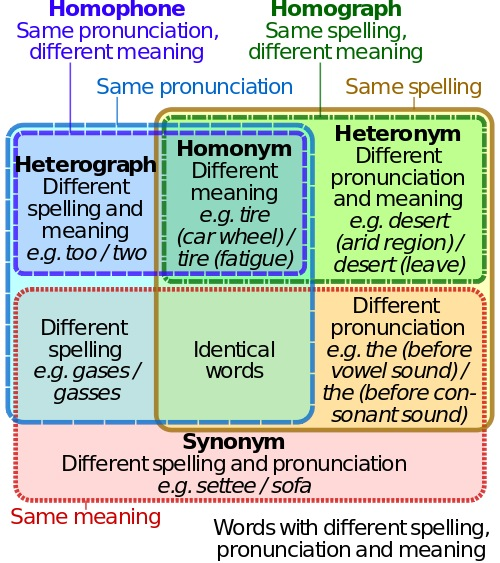
\includegraphics[width=0.5\textwidth]{500px-Homograph_homophone_venn_diagram.jpg}
\captionfonts
\caption[Word Categorization Venn Diagram]{A word categorization Venn Diagram that shows the different terms for variations in word spelling, pronunciation, and meaning. }
\label{fig:vocab:wordCategorizationDiagram}
\end{figure}

\subsection{Homographs}
\label{section:Homographs}


Homographs are orthographic words that are spelled identically. Typically, homographs are also pronounced differently, which makes them homographic heterophones(~\ref{fig:vocab:wordCategorizationDiagram}). For example, there are two homographs for the word ``does, because it has two different pronunciations: the ``multiple female deer'' does (doze), and the ``third-person singular present indicative form of `do' '' does (duhz). If the words are spelled identically AND pronounced identically, then then are homographic homophones, which are commonly known as homonyms.


\subsection{Heterographs}
\label{section:Heterographs}

Heterographs are orthographic words that are spelled differently. Typically, words are only called heterographs if they are also pronounced differently, making them heterographic homophones. Most words in the English language are heterographic heterophones; that is, spelled and pronounced uniquely. Because this is the default state of a word set, we rarely describe such words in terms of homo\slash hetero phones\slash graphs.  As such, the only time a word set is likely to be described as heterographic is if it is also a homophone. For example, the banes of every grammarian, ``there'', ``their'', and ``they're'', are heterographic homophones. Alternatively, ``to'', ``too'', and ``two'' are also heterographic homophones.  

\subsection{Homophones}
\label{section:Homophones}

Homophones are orthographic words that are pronounced identically, but typically spelled differently. If a homophone set is also homographic (that is, spelled identically as well as pronounced identically), then we refer to them as homonyms. As such, the only time the words in a set are likely to be labelled ``homophones'' is if they are also heterographic.

\subsection{Homonyms}
\label{section:Homonyms}

Homonyms are orthographic words that are pronounced and spelled identically, but defined differently. For example, depending on context, the word ``left'' can mean left (the opposite of right), or left (the past tense of leave). Homonyms can also be referred to as homographic homophones.


\section{Phonetics and Phonology}
\label{vocab:phoneticsAndPhonology}
To discover oronyms for a phrase, we must first to translate the root orthographic phrase to a representation that allows us to unambiguously measure pronunciation.   Phonology and phonetics are branches of linguistics that deal with pronunciation.

\subsection{Phonetics}
\label{vocab:phonetics}
Phonetics is a branch of \emph{descriptive} linguistics, and refers to the study of the actual, uttered sound of human speech. It deals with describing the physical phenomena of how these sounds are produced from the vocal tract, how they are transmitted once spoken, and how they are recieved by audiences. The building blocks of phonetics are \emph{phones}, which represent atomic sounds.

\subsection{Phonology (aka phonemics)}
\label{vocab:phonology}
Phonology is a branch of \emph{theoretical} linguistics, and as such, is primarily concered with the abstract grammatical characterization of sounds.  It describes the way that sounds function within a language to give meaning to words.  The basis of phonological analysis is the grouping of sounds (\emph{phones}) into distinct units within a languages.  These distinct units are called \emph{phonemes}.  

These phonemes may contain different phones, depending on the accent of the speaker.  For example, native speakers of General American English only generally recognize one `L' sound phoneme. However, there are two different ways that that phoneme manifests itself: the `l' in ``male", and the `l' in late. This difference is not noticable to a native speaker of American English, because that particular accent will parse any `L' phone as the same `L' phoneme. It would, however, be recognizable to someone whose accent categorizes those phones into two separate phonemes.

\subsection{Phonetics Vs Phonology}
\label{vocab:phoneticsVsPhonemics}

Though the terms are sometimes used interchangably, the words `phonemic' and `phonetic' (and their corresponding sound building blocks, `phone' and `phoneme')  indicate different stages of sound parsing.  \emph{Phonemes} are idealized sounds; \emph{phones} are the actual sounds that come out of a person's mouth.  Figure ~\ref{fig:knightsPhoneticPhonemic} provides a final, illustrative metaphor of the difference.
%\begin{center}
\begin{figure}[b]
\centering
        \begin{subfigure}[b]{0.4\textwidth}
                \centering
                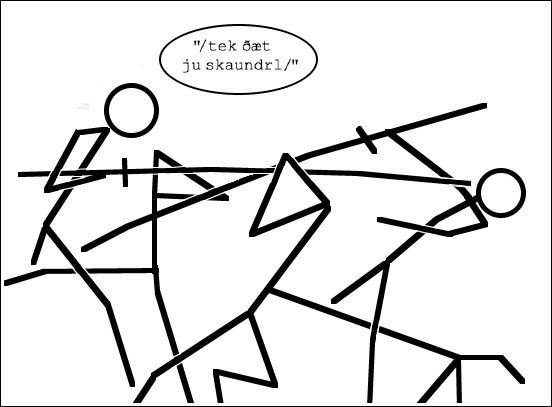
\includegraphics[width=\textwidth]{knights_phonemic.jpg}
                \captionfonts
                \caption[Phonemic Knights]{Phonology\cite{cartoonPhonemic} }
                \label{fig:cartoonPhonemic}
        \end{subfigure}
        \quad
        \begin{subfigure}[b]{0.4\textwidth}
                \centering
                
\includegraphics[width=\textwidth]{knights_phonetic.jpg}
                \captionfonts
                \caption[Phonetic Knights]{Phonetics\cite{cartoonPhonetic} }
                \label{fig:cartoonPhonetic}
        \end{subfigure}
\caption{The difference between phonetics and phonology}\label{fig:knightsPhoneticPhonemic}
\end{figure}
%\end{center}    

\FloatBarrier

\section{Phonemic/Phonetic Alphabets}
\label{section:phonemicAlphabets}
\begin{wrapfigure}{r}{0.5\textwidth}
\begin{center}
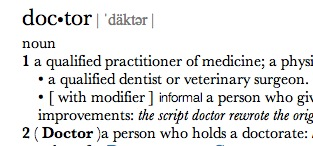
\includegraphics[width=70mm]{doctorDictIPAScreenshot.jpg}
\captionfonts
\caption[Dictionary IPA screenshot]{ The characters to the right of the large bold word ``doctor" are IPA symbols. }
\label{fig:doctorDictIPAScreenshot}
\end{center}
\end{wrapfigure}

As we stated in section~\ref{vocab:phonology}, phonemes are the atomic building blocks of words. In a phonemic alphabet, every meaningful sound has its own ``letter''.  The way that we interact with phonemes in a concrete, textual way is by using phonetic alphabets and phonetic dictionaries.  

The most common phonetic alphabet is the IPA (International Phonetic Alphabet). It contains representations of every sound in every known language globally, and allows for cross-cultural pronunciation guidelines.  As shown in figure~\ref{fig:doctorDictIPAScreenshot}, IPA representations of orthographic words are found in traditional dictionaries to aid pronunciation. 

\subsection{SAMPA}
\label{section:sampaAlphabet}

SAMPA (Speech Assessment Methods Phonetic Alphabet) is a computer-readable phonetic alphabet, based upon the symbols found in the more-standard-but-not-easily-computer-readable  IPA (International Phonetic Alphabet).  
It uses ``letters" consisting of 1-2 ASCII characters to represent each phoneme. The ASCII sequences corresponding to each of the SAMPA letters are designed so that any SAMPA sequence is deterministically parsible.

We chose to use SAMPA instead of IPA because its ASCII-compliance makes it easy to integrate into other systems.

See the table in appendix ~\ref{appendix:table:sampaTable} for a full table of each SAMPA phoneme, its description, and its sub-parts.

For some brief examples, the SAMPA spelling of the name `Jenee Hughes' is \emph{dZEni hjuz}.  
`Dr Zoe Wood'  becomes \emph{dAkt@\char18r zoui wUd}.  
`Dr John Clements' becomes \emph{dAkt@\char18r dZAn klEm@nts}. 
`Dr Franz Kurfess' becomes \emph{dAk@\char18r fr\{nz k3\char18rfEs}.

